% =============================================================================
% CAPÍTULO 4 — volta 1 (AGENTS.md §6): o orçamento do alarme.
%
% O fracasso que o abre, com número na mão: o vigia do capítulo 3, ligado no limiar que o
% mundo parado não ultrapassa, soa uma vez a cada 3632 anos de mundo parado e avisa do
% tombo de 2020 com 86% do prejuízo já pago. A troca entre silêncio e antecedência é a
% curva da fig:troca; o atraso tem piso provado (prop:piso); o orçamento se compra com
% memória (1/(n+1)) — e a forma da mudança, que decide o preço desse silêncio, é o capítulo
% seguinte.
%
% Medição: lab/experimentos/E02_orcamento.ipynb. Figuras: figuras/E02_orcamento_1 e _2.
% =============================================================================

\chapter{O orçamento do alarme}
\label{cap:orcamento}

\section{O vigia}

O capítulo anterior deixou um instrumento e um incômodo. O instrumento conta quantas vezes o
preço rompeu a linha dentro de uma janela móvel de \numVigiaBloco{} dias. O incômodo é que os
blocos têm data: a contagem sobe nos mesmos anos, e sobe sempre no mesmo lugar da série.

A tentação, agora, é pequena e razoável. Se o bloco sabe \emph{quando} o mundo aperta, basta
ligar nele um alarme: soa quando a contagem passa de um limiar. E o limiar já vem escolhido
por medição, não por gosto, porque no capítulo anterior o pior bloco de duzentos mundos que
nunca mudam chegou a \numNuncaMudaPiorBloco{} violações. Um número que o mundo parado não
ultrapassa é um candidato honesto a linha de alarme --- e \numVigiaMundosQueSoamPct\% dos mundos
parados o alcançam, um em cada duzentos.

Fica então o vigia mais simples que dá para escrever: \emph{soa quando as violações dos
últimos \numVigiaBloco{} dias chegam a \numVigiaLimiar}.

Duas perguntas decidem se isso vale alguma coisa, e o capítulo é sobre elas: com que
frequência ele soa quando nada muda, e quanto tempo ele leva quando algo muda de verdade. As
duas precisam de resposta junta, porque cada uma é paga com a outra \cite{wald1945sequential}.

\section{Quanto ele soa quando nada muda}

% aterramento: falso-alarme
A primeira pergunta não se responde no mercado, porque no mercado não se sabe quais alarmes
eram falsos. Sabe-se que houve alarme, e só. O alarme que soa num mundo que não mudou tem nome
--- é o \textbf{falso alarme} ---, e a frequência com que ele soa é o orçamento do vigia.
Responde-se em mundos em que nada muda:
\numVigiaMundos{} séries do tamanho da nossa, com retornos independentes e sempre a mesma
lei, submetidas ao mesmo corte, aos mesmos blocos e ao mesmo limiar.

No limiar \numVigiaLimiar{}, essas mil séries produziram \numVigiaDiasParadoPorMundo{} dia de
alarme por mundo --- quase nada ---, e \numVigiaMundosQueSoamPct\% dos mundos soaram pelo
menos uma vez ao longo de vinte e cinco anos. Dito em tempo: o vigia soa sozinho uma vez a
cada \numVigiaAnosParadoPorAlarme{} anos.

Um número desses pede desconfiança, e a desconfiança aqui é aritmética. Ele se apoia em
\numVigiaParadoAlarmes{} alarmes espalhados por \numVigiaMundos{} mundos; contar evento raro
é impreciso, e o erro relativo dessa contagem é de \numVigiaParadoErroPct\%. O que a medição
entrega é a ordem de grandeza --- milhares de anos ---, e não o número exato.

Há um jeito de conferir esse orçamento sem sortear nada, e ele cabe numa proposição, porque a
conta é uma união de acontecimentos.

% aterramento: prob
% aterramento: A
% aterramento: binomial
% aterramento: B
% aterramento: L
Escrevo $\Prob(A)$ para a probabilidade do acontecimento $A$. Falta nomear as peças do bloco:
ele tem $B$ dias, cada um com a probabilidade $p$ de violar o corte, e o alvo é $L$ violações.
A contagem dentro de um bloco de $B$ dias independentes é a soma de $B$ indicadores --- o mesmo indicador
do dia que a barra da média usou ---, de modo que a chance de ela alcançar $L$ é a cauda dessa soma, que se escreve
$\Prob\big(\text{Bin}(B, p) \geq L\big)$ e se lê assim: a probabilidade de a contagem de
$B$ sorteios independentes, cada um com probabilidade $p$, chegar a $L$.

\begin{proposicao}[o teto independente]
\label{prop:teto}
Se os dias fossem independentes, com probabilidade $p$ de violar o corte em cada dia, então a
probabilidade de algum bloco de $B$ dias atingir $L$ violações não passaria de
$n \cdot \Prob\big(\text{Bin}(B, p) \geq L\big)$, onde $n$ é o número de blocos.
\end{proposicao}

\begin{proof}
O acontecimento \emph{algum bloco atinge o limiar} é a união, sobre os $n$ blocos, dos
acontecimentos \emph{este bloco atinge o limiar}. A probabilidade de uma união nunca excede a
soma das probabilidades dos seus termos, e sob independência a probabilidade de um bloco
atingir $L$ violações é a cauda da binomial.
\end{proof}

Com os números do vigia o teto dá \numVigiaTetoIndependentePct\%, e o mundo parado
mediu \numVigiaMundosQueSoamPct\%. O teto está acima do medido, como tinha de estar, e está
acima por quase uma dezena de vezes: é um limite provado e frouxo, e vale pelo que prova.

Ele também tem prazo de validade, e o prazo aparece na própria conta. Para limiares baixos a
soma das parcelas ultrapassa cem por cento, e um teto que passa de cem por cento não é teto de
nada.

\section{Quanto ele demora quando algo muda}

O orçamento sozinho não decide nada. A pergunta que decide é a outra: quando o mundo muda, o
vigia avisa a tempo de quê?

Na série inteira, e no mesmo limiar, ele soou \numVigiaAlarmesReais{} vezes em vinte e cinco
anos, uma a cada \numVigiaAnosReaisPorAlarme{} anos. No mundo parado o mesmo vigia soa uma vez
a cada \numVigiaAnosParadoPorAlarme{} anos, ou \numVigiaRazaoRealContraParado{} vezes mais
raro. Quem soa uma vez a cada três anos e meio num mundo que muda está respondendo ao mundo, e
não ao próprio ajuste.

Para medir a que ele responde, cada alarme é comparado com o topo anterior e o fundo seguinte
--- o preço mais alto antes do tombo e o mais baixo depois ---, e a conta que interessa é
quanto do prejuízo total já tinha acontecido no dia do aviso.

Nos dois tombos maiores do período, o resultado é este.

\begin{table}[htbp]
  \centering
  \begin{tabular}{lrrr}
    \hline
    & atraso desde o topo & prejuízo já pago \\
    \hline
    alarme de \numVigiaTomboAntigoData & \numVigiaTomboAntigoAtrasoDias{} dias & \numVigiaTomboAntigoPagoPct\% \\
    alarme de \numVigiaTomboRecenteData & \numVigiaTomboRecenteAtrasoDias{} dias & \numVigiaTomboRecentePagoPct\% \\
    \hline
  \end{tabular}
  \caption{Os dois piores tombos do período, com o dia do alarme e a fração do prejuízo total
    que já tinha acontecido quando ele soou. No tombo mais recente, o alarme veio com
    \numVigiaTomboRecenteQuedaPct\% de queda já realizada, de um total de
    \numVigiaTomboRecenteTotalPct\%.}
  \label{tab:atraso}
\end{table}

A mediana dos \numVigiaAlarmesReais{} alarmes é de \numVigiaPagoMedianoPct\% de prejuízo já
pago. Num deles o alarme soou no fundo exato, com \numVigiaPagoPiorPct\% do tombo consumido:
o vigia avisou no dia em que a queda acabou.

Vale dizer do modo mais direto possível. O vigia acerta: os alarmes dele são reais, e o mundo
parado quase nunca o faz soar. O que ele não faz é chegar antes.

\section{A troca}

Se o vigia é tardio, a saída parece óbvia: baixar o limiar. Baixar o limiar antecipa o alarme
e cobra por isso, e o que vale medir é quanto, porque o preço tem forma.

Para cada limiar medimos as duas coisas de uma vez: a frequência com que ele soa em mundo
parado, e quanto do prejuízo já estava pago quando ele soou no tombo recente.

\begin{table}[htbp]
  \centering
  \begin{tabular}{rrr}
    \hline
    limiar & um alarme falso a cada & prejuízo já pago no tombo recente \\
    (violações) & (anos de mundo parado) & (\%) \\
    \hline
    \numTrocaOitoLimiar & \numTrocaOitoAnos & \numTrocaOitoPagoPct \\
    \numTrocaNoveLimiar & \numTrocaNoveAnos & \numTrocaNovePagoPct \\
    \numTrocaDezLimiar & \numTrocaDezAnos & \numTrocaDezPagoPct \\
    \numTrocaOnzeLimiar & \numTrocaOnzeAnos & \numTrocaOnzePagoPct \\
    \numTrocaDozeLimiar & \numTrocaDozeAnos & \numTrocaDozePagoPct \\
    \numVigiaLimiar & \numTrocaTrezeAnos & \numTrocaTrezePagoPct \\
    \hline
  \end{tabular}
  \caption{A troca, medida. Baixar o limiar antecipa o alarme e multiplica o falso alarme; a
    taxa de câmbio não é constante, e piora à direita da tabela.}
  \label{tab:troca}
\end{table}

A tabela diz três coisas.

\textbf{A troca existe, e o primeiro passo é barato.} Baixar o limiar de \numVigiaLimiar{}
para \numTrocaOitoLimiar{} derruba o prejuízo já pago de \numTrocaTrezePagoPct\% para
\numTrocaOitoPagoPct\%: o vigia passa a avisar antes de o tombo se completar.

\textbf{O preço desse passo é brutal.} O mesmo movimento leva o falso alarme de um a cada
\numTrocaTrezeAnos{} anos de mundo parado para um a cada \numTrocaOitoAnos{} anos. O vigia que
quase nunca se enganava passa a soar a cada poucos anos sem que nada tenha mudado.

\textbf{E a taxa de câmbio piora na outra ponta.} Do limiar \numTrocaDezLimiar{} para o
\numTrocaDozeLimiar, o falso alarme fica quase vinte vezes mais raro e o prejuízo já pago sobe
de \numTrocaDezPagoPct\% para \numTrocaDozePagoPct\%: trinta pontos de prejuízo comprados com
silêncio. E há dois limiares vizinhos entregando quase a mesma coisa --- o \numTrocaDozeLimiar{} e o
\numVigiaLimiar, com \numTrocaDozePagoPct\% contra \numTrocaTrezePagoPct\%.

\begin{figure}[htbp]
  \centering
  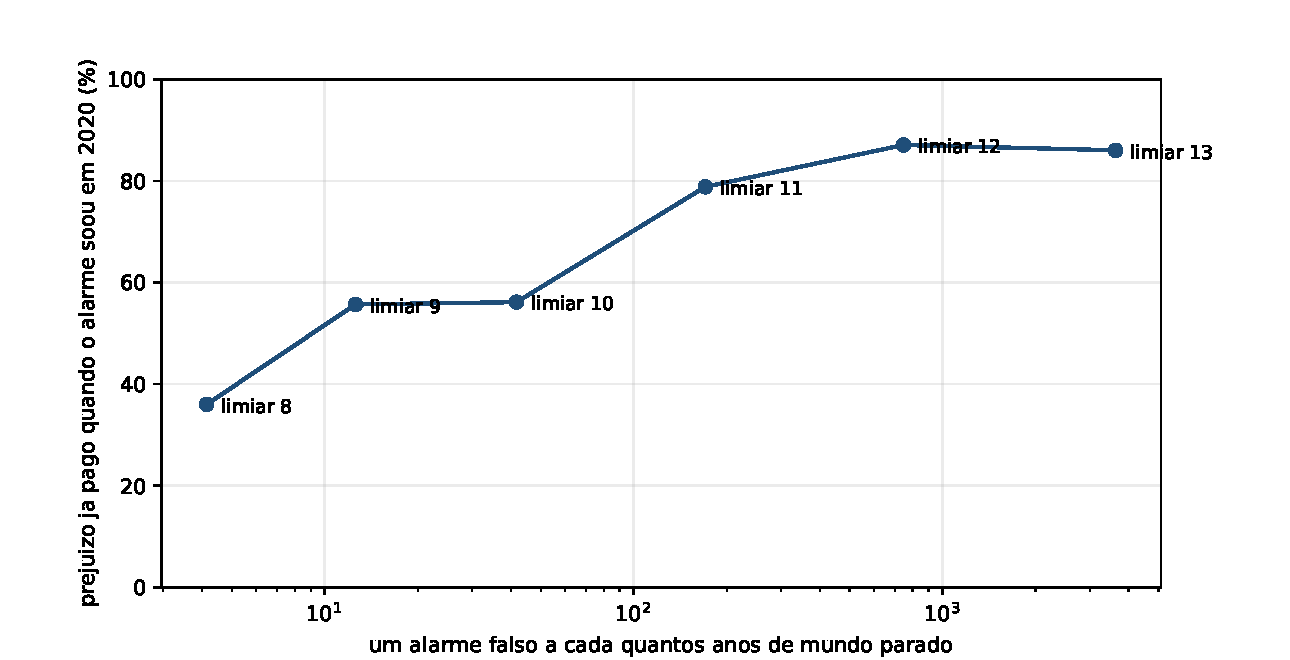
\includegraphics[width=\linewidth]{figuras/E02_orcamento_1.pdf}
  \caption{A troca em forma de curva: o eixo horizontal é a raridade do falso alarme, em
    escala logarítmica, e o vertical é o prejuízo já pago no tombo recente. A curva sobe
    depressa na esquerda e achata na direita.}
  \label{fig:troca}
\end{figure}

Não existe limiar que seja ao mesmo tempo raro e rápido. O vigia é o par --- frequência em
mundo parado e atraso em mundo que muda ---, e escolher um limiar é escolher um ponto dessa
curva, com o preço da esquerda pago em falso alarme e o da direita pago em atraso.

\section{O piso}

Antes de concluir que o vigia está mal calibrado, vale olhar o chão em que ele está, porque o
atraso dele tem piso, e o piso é aritmético.

\begin{proposicao}[o piso do atraso]
\label{prop:piso}
Um alarme que exige $L$ violações dentro da janela móvel não pode soar antes de $L-1$ pregões
depois de a mudança começar, se antes dela o corte não era violado.
\end{proposicao}

\begin{proof}
Para que a contagem chegue a $L$, são necessários ao menos $L$ dias com violação dentro da
janela. Cada dia com violação consome um pregão, e nenhum deles pode ser anterior ao começo da
mudança --- que é um dia mudado, e já pode violar. Contando o dia da mudança como zero, o alarme
não pode soar antes de $L-1$ pregões.
\end{proof}

Com $L = \numVigiaLimiar$, o piso é de \numVigiaPisoPregoes{} pregões. O alarme de
\numVigiaTomboRecenteData{} soou \numVigiaTomboRecenteAtrasoDias{} dias corridos depois do
topo: o vigia não estava gastando tempo à toa, estava
esperando a contagem encher, que é o que ele sabe fazer.

A consequência é dura para quem queria melhorar o vigia ajustando números. A única alavanca é
o próprio limiar, e o limiar é o orçamento; comprar velocidade é pagar em falso alarme, na
taxa de câmbio da \cref{tab:troca}.

\begin{figure}[htbp]
  \centering
  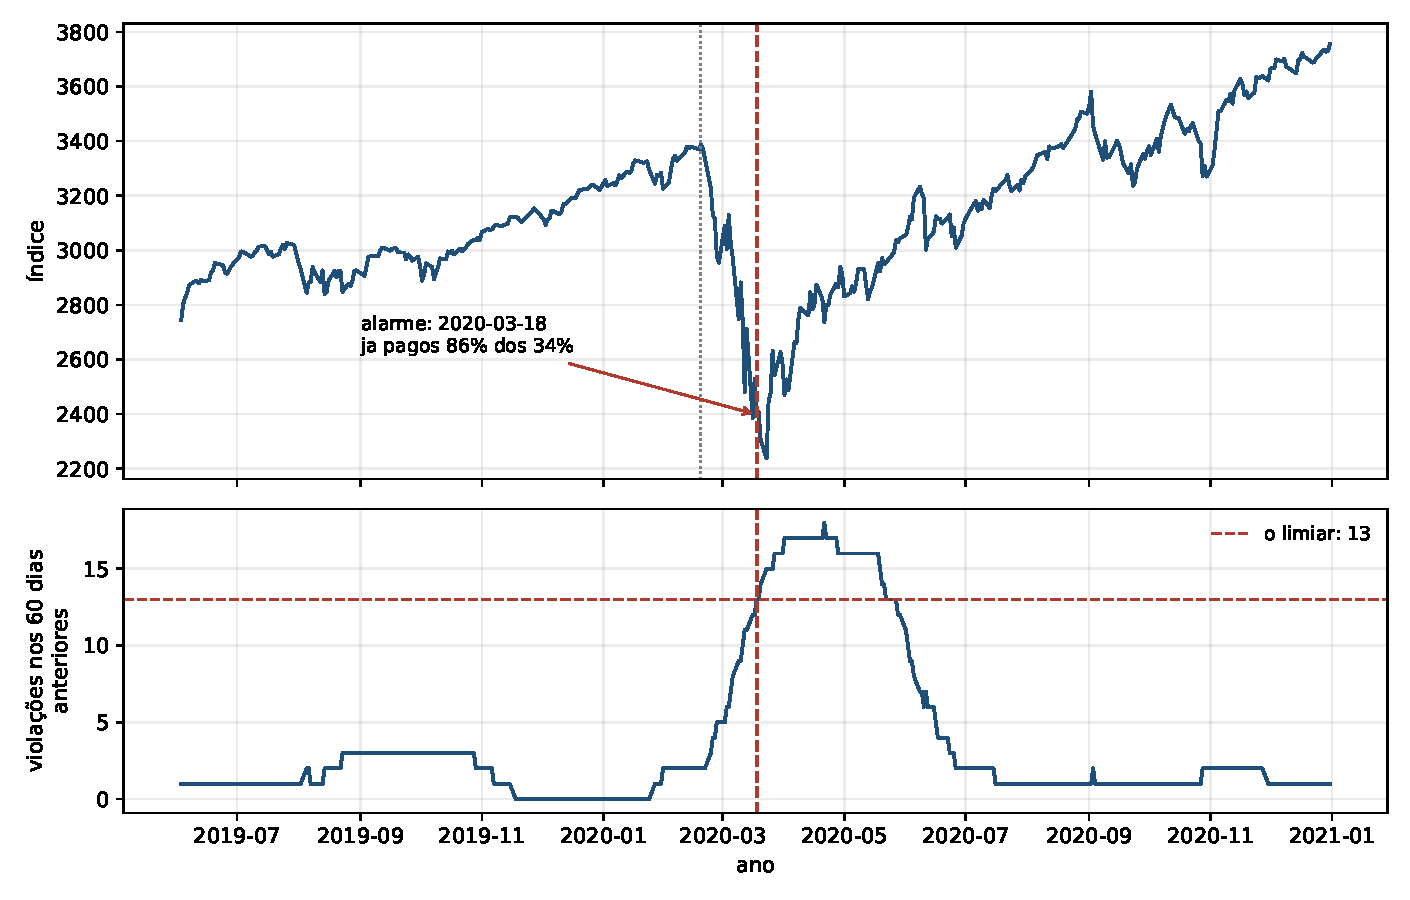
\includegraphics[width=\linewidth]{figuras/E02_orcamento_2.pdf}
  \caption{O alarme de \numVigiaTomboRecenteData{} visto dos dois lados. Em cima, o índice;
    embaixo, as violações dos \numVigiaBloco{} dias anteriores, com o limiar. As duas linhas
    contam a mesma história --- e a de baixo conta depois da de cima.}
  \label{fig:vigia2020}
\end{figure}

\section{O mesmo corte, lido mais fundo}

Tudo o que foi medido até aqui é uma leitura do corte do capítulo anterior: contar quantas
vezes o preço rompeu a linha, e alarmar quando a contagem enche. O corte admite uma segunda
leitura, mais direta, e vale olhá-la antes de aceitar que o vigia é assim mesmo.

Nessa leitura o alarme não espera contagem nenhuma. Ele soa no dia em que o preço fica abaixo
do $k$-ésimo pior dos últimos $n$ dias; com $k = 1$, soa no dia em que o preço faz o pior dia
do último ano. É o mesmo corte, com o posto escolhido de outro jeito, e dessa vez a escolha
tem conta fechada, porque é a proposição do capítulo anterior lida ao contrário: o posto $k$
com janela $n$ assina a taxa $k/(n+1)$.

Isso muda a natureza do orçamento. Na leitura do bloco, a frequência do falso alarme não tem
forma fechada --- sessenta blocos móveis se sobrepõem, e o melhor que se consegue é medir, com
o erro de contagem que a \cref{prop:teto} limita por cima. Na leitura do dia a frequência é
exata, e o número declarado é o número entregue: nos mundos que nunca mudam, a medição
devolveu \numSegundaLeituraParadoAlarmes{} alarmes contra os \numSegundaLeituraParadoDeclarado{}
que a conta declara.

Daí sai um limite que calibração nenhuma contorna. O posto mais fundo possível é o primeiro da
fila, de modo que com $n$ dias de memória --- e aqui \textbf{memória} é o nome do que se compra:
quantos dias o alarme olha para trás --- o alarme mais raro que existe é $1/(n+1)$.
% aterramento: memoria-janela
Um alarme
por ano custa \numMemoriaUmAlarmePorAnoDias{} dias de memória; um alarme por década custa
\numMemoriaUmAlarmePorDecadaDias{} dias, que são dez anos de série, e quem não tem esses dias
não tem esse alarme.

O que essa leitura compra é tempo. No orçamento de \numFundoUmAnoAlarmesPorAno{} alarme por
ano, ela avisou do tombo recente em \numSegundaLeituraTomboRecenteData, com
\numSegundaLeituraTomboRecentePagoPct\% do prejuízo já pago, contra os
\numVigiaTomboRecentePagoPct\% da leitura do bloco. No tombo antigo, avisou em
\numSegundaLeituraTomboAntigoData{} com \numSegundaLeituraTomboAntigoPagoPct\%, contra
\numVigiaTomboAntigoPagoPct\% da outra leitura.

A comparação, porém, pede cuidado, porque os dois vigias foram declarados em orçamentos
diferentes: \numFundoUmAnoAlarmesPorAno{} alarme por ano de um lado, um a cada
\numVigiaAnosParadoPorAlarme{} anos do outro. No ponto em que os dois orçamentos se aproximam,
a vantagem some. Com \numFundoCincoAnosAlarmesPorAno{} alarme por ano, ou um a cada cinco
anos, a leitura do dia chegou ao tombo recente em \numSegundaLeituraCincoAnosTomboRecenteData{}
com \numSegundaLeituraCincoAnosTomboRecentePagoPct\% do prejuízo pago; a leitura do bloco, no
limiar \numTrocaOitoLimiar, soa uma vez a cada \numTrocaOitoAnos{} anos e chega com
\numTrocaOitoPagoPct\%. Duas leituras do mesmo corte, silêncios próximos e quase o mesmo preço.

E a leitura do dia tem um preço próprio, que a tabela do bloco não mostra. Num mundo que nunca
muda ela soa, por construção, na taxa que declarou: a conta pede
\numSegundaLeituraParadoDeclarado{} alarmes e a medição devolveu \numSegundaLeituraParadoAlarmes{}.
Na série real foram \numSegundaLeituraAlarmesReais{}, ou \numSegundaLeituraAlarmesAno{} por ano,
contra o \numFundoUmAnoAlarmesPorAno{} declarado --- enquanto o vigia do bloco soou
\numVigiaAlarmesReais{} vezes no mesmo período. A escolha é entre um vigia que fala \numSegundaLeituraAlarmesAno{}
vezes por ano e chega cedo, e um vigia que fala uma vez a cada três anos e meio e chega depois.

\section{O que fica}

O que fica é o orçamento, e ele fixa uma coisa só: \textbf{todo alarme é um par declarado} ---
com que frequência ele soa quando nada muda, e quanto ele demora quando algo muda. Um alarme que não declara o par não é uma afirmação; é barulho com opinião. Fica também
a moeda do par: ele se compra com memória, porque o alarme mais raro que $n$ dias de janela
permitem é $1/(n+1)$, e se paga conforme a forma da mudança, que decide quantos dias custa
sair do silêncio.

E fica o fracasso seguinte, que a curva da troca não mostra: ela foi medida com os tombos do
mercado, e o tombo é a forma de mudança mais fácil de ver. O mundo muda de outras maneiras.
